\title{Riassunto Pugliese}
\author{
        Tommaso Puccetti \\
                Studente presso Universita degli studi di Firenze
}
\date{\today}

\documentclass[12pt]{article}
\usepackage{graphicx}
\usepackage{hyperref}

\begin{document}
\maketitle
\tableofcontents
\listoftables
\listoffigures
\section{Overview}
	\subsection{Computer Security Concepts}
		\textbf{Computer security }: \textit{ La protezione fornita ad un sistema informatico automatizzato con lo scopo di raggiungere gli obiettivi applicabili di preservare \textbf{integrity}, \textbf{availability}, \textbf{confidentiality} , delle risorse del sistema (include hardware, software, firmware, informazioni/dati, telecomunicazioni).}  (NIST Computer Security Handbook 1995)\\
		\subsubsection{CIA triad: tre obiettivi per la sicurezza}
			\begin{itemize}
				\item \textbf{Confidentiality} questo termine copre due concetti a esso correlati 
				\begin{enumerate}
					\item \textbf{Data confidecntiality}: Assicura che informazioni confidenziali non siano rilasciate ad individui non autorizzati.
					\item \textbf{Privacy}: Assicura all'individuo la possibilita di controllare od influenzare quali informazioni a loro relative possono essere raccolte e salvate, a chi e permesso raccoglierle e a chi potrebbero essere rilasciate.
				\end{enumerate}
				\item \textbf{Integrity}:
				 \begin{enumerate}
					\item \textbf{Data integrity}: assicurare che le informazioni e i programmi sono modificati solo in modo specificato ed autorizzato
					\item \textbf{System integrity}: assicurare che il sistema esegue le sue operazioni in modo non corrotto, senza che vi siano manipolazioni non autorizzate.
				\end{enumerate}
				\item \textbf{Availability}: Assicura che il sistema fornisce i suoi servizi prontamente, senza che il loro accesso sia negato ad utenti non autorizzati. (In QAS percentuale di tempo in cui il sistema e funzionante rispetto alla vita operazionale totale del sistema.)
			\end{itemize}
			Si hanno ulteriori concetti complementari a quelli sopra elencati:
			\begin{itemize}
				\item \textbf{Authenticity}: assicura che un'entita o un oggetto è genuino e fidato. Deve esserci la possibilià di essere verificato. \textit{Supporta la confidence riguardo alla validità di una trasmissione, di un messaggio o del suo creatore}
				\item \textbf{Accountability}: Assicura che le azioni di una particolare entità siano attribuibili unicamente a quell'entità.\textit{Supporta nonrepudiation, intrusion detection, prevention, fault isolation ecc}.
			\end{itemize}	
		\subsubsection{Livelli di impatto riguardo a breccie nella sicurezza}
			\begin{itemize}
				\item \textbf{Low}: la perdita di sicurezza informazioni ha un impatto limitato ( una degradazione rispetto alla mission del sistema, danno minimo, minima perdita finanziaria, minaccia  )
				\item \textbf{Moderate}: la perdita a effetti seri (significativa degrado rispetto alla missione del sistema, minaccia significativa verso individui senza che sia a rischio la vita o siano considerabili infortunei che mettono a rischio la vita di un individuo.)
				\item \textbf{High}: la perdita di sicurezza ha severi o catastrofici effetti collaterali riguardo le operazioni, asset organizzativi o individui (perdita della vita).
			\end{itemize}
		\textbf{Esempio Confidentiality}:\\
			La confidentiality dei voti ottenuti da uno studente è considerata essere \textbf{molto importante}. Per quanto riguarda, invece, le informazioni riguardo la sua immatricolazione, possiamo dire che hanno un tasso di confidentiality piu basso. La lista degli studenti ha un tasso ancora minore.		\\
		\textbf{Esempio Integrity:}\\
			Informazioni riguardo le allergie di un paziente, richiedono requisiti alti di integrità ( un dottore deve poter ritenere affidabili le informazioni che riceve up to date. Se qualcuno falsifica deliberatamente i dati il database dobrebbe essere ripristinato ad una base fidata e si dovrebbe poter associare le informazioni falsificate a chi ha commesso tale falsificazione.)
			Se consideriamo le informazioni di una newsgroup queste hanno dei requisiti di integrità più bassi.
			Ancora meno ne hanno i sondaggi anonimi online. \\
		\textbf{Esempio Availability:}
		Un sistema che fornisce un servizio di autenticazione a sistemi critici, applicazioni o dispositivi. In questo caso abbiamo possibili perdite finanziarie e dunque la necessità di avere alti requisiti di availability. Se consideriamo il sito web di una università, l'interruzione del servizio causa imbarazzo, ma nessun danno critico. Dunque si hanno requisiti più bassi di availability. Infine un elenco telefonico online che non è consultabile al massimo crea disagio, ma ci sono comunque fonti alternative per questo tipo di informazioni, bassi requisiti di availability.
		
		\subsubsection{Sfide riguardo la sicurezza dei computer}
			\begin{enumerate}
				\item La sicurezza dei computer non è semplice;
				\item Si devono considerare potenziali (inattesi ) attacchi;
				\item Le procedure utilizzate sono spesso controintuitive;
				\item Dobbiamo decidere dove inserire (deploy) meccanismi di difesa;
				\item Include algoritmi e informazioni segrete (keys);
				\item COMPLETARE L?ELENCO  
			\end{enumerate}
			
		\subsubsection{Un modello per la sicurezza dei computer}
			Gli utenti ed i proprietari vogliono proteggere gli \textbf{asset}, o risorse del sistema: Hardware, software (OS, apps), data (users, system, database), communication facilities and networks (LAN, bridges, routers, ...).\\
			Le nostre preoccupazioni riguardano le \textbf{vulnerabilità} di queste risorse (sottratte, danneggiate, non disponibili).
			Le minacce evidenziano vulnerabilità e rappresentano potenziali danni nei confronti di un \textbf{asset}. \\
			Un \textbf{attacco} è una minaccia che è portata avanti da un \textbf{attaccante} (or \textbf{threat agent}). 	
			\begin{itemize}
				\item \textbf{Attacco attivo:} un tentativo di alterare le risorse del sistema o di influenzare le sue operazioni.
				\item \textbf{Attacco passivo:} un tentativo di imparare o fare uso di informazioni provenienti dal sistema, senza influenzarne le risorse.
				\item \textbf{Attacco dall'interno:} iniziato da un'entità all'interno del perimetro di sicurezza.
				\item \textbf{Attacco dall'esterno:} iniziato da un'entità al di fuori del perimetro di sicurezza, da parte di un utente non autorizzato o illegittimo.
			\end{itemize}
			 Per \textbf{contromisure} intendiamo tutte le azioni intraprese per prevenire, rilevare, ripristinare o minimizzare un rischio che riguardi un asset del sistema. \\
			 \textit{Segue figure:\ref{fig:1}}
			 \begin{figure}[h!]
			 	\centering
			 	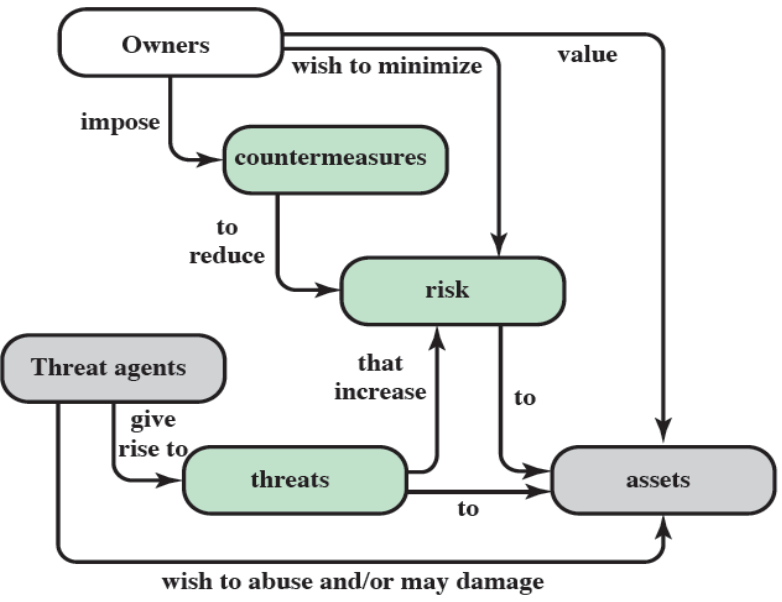
\includegraphics[scale=0.40]{img/securityrel.PNG}
			 	\caption{Security concepts and relationships\label{fig:1}}
			 \end{figure}
			 
		\subsection{Minacce, attacchi e asset}
			\subsubsection{Minacce, conseguenze ed attacchi}
				\begin{itemize}
					\item \textbf{Rilascio non autorizzato (unauthorized disclosure):} minaccia la confidentiality.
					\begin{itemize}
						\item Una circostanza o un evento nel quale un'entità non autorizzata guadagna l'accesso a dati per i quali non sarebbe autorizzato.
						\item Ad esempio rilascio, intercettazione o inferenza di dati sensibili.
					\end{itemize}
					\item \textbf{Inganno (deception):} minaccia l'integrità.
					\begin{itemize}
						\item Circostanza o evento nel quale un'entità autorizzata riceve dati falsificati credendo che siano corretti.
						\item Può essere il caso di un utente non autorizzato che si finge utente autorizzato (\textbf{masquerade}). Si includono venti relativi alla falsificazione (\textbf{alter data}) o al falso diniego della responsabilità nei confronti di uno specifico atto (\textbf{repudation}).
					\end{itemize}
					\item \textbf{Rottura (disruption):} minacce ad integrità e availability.
					\begin{itemize}
						\item Circostanza o evento che interrompe il funzionamento o i servizi del sistema.
						\item Ad esempio disabilitare una componente del sistema (\textbf{incapacitation}), modificare in modo negativo le funzioni del sistema o i suoi dati (\textbf{corruption}), o intasare (overload) una linea di comunicazione \textbf{obstruction} 
					\end{itemize}
					\item \textbf{Usurpazione}: minaccia all'integrità.
					\begin{itemize}
						\item Circostanza nella quale un'entità non autorizzata prende il controllo di una funzione o servizio del sistema.
						\item Furto di un servizio (\textbf{misappropriation}), hacker che guadagnano un accesso non autorizzato (\textbf{misuse}.)
					\end{itemize}
				\end{itemize}
				 \textit{Segue figure:\ref{fig:2},\ref{fig:3},\ref{fig:4}}
				\begin{figure}[h!]
					\centering
					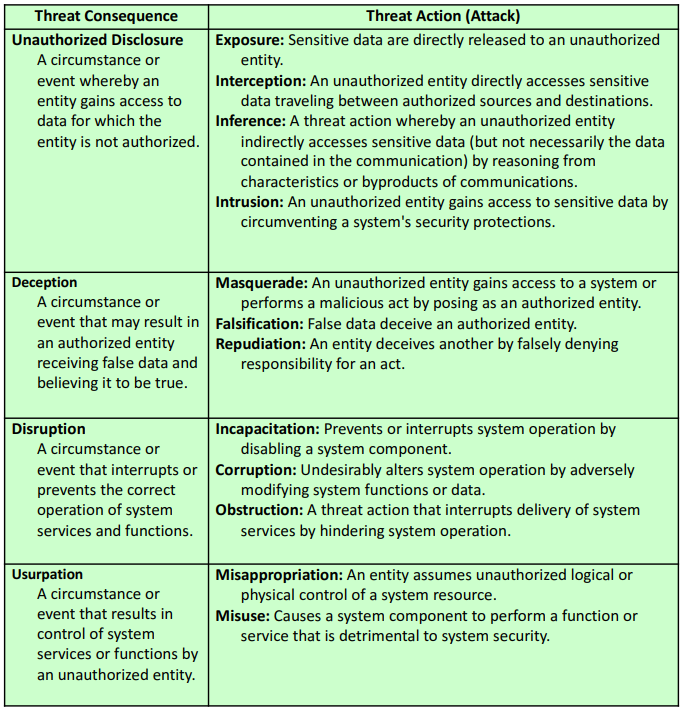
\includegraphics[scale=0.60]{img/threat.PNG}
					\caption{Threat consequences and attack\label{fig:2}}
				\end{figure}
				\begin{figure}[h!]
					\centering
					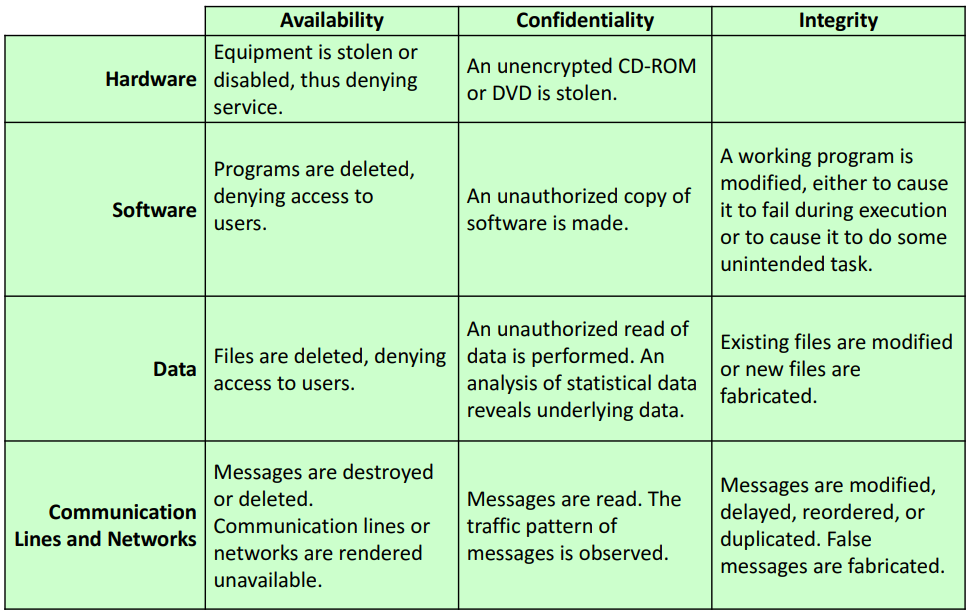
\includegraphics[scale=0.40]{img/asset.PNG}
					\caption{Examples	of	threats	to	assets\label{fig:3}}
				\end{figure}
				\begin{figure}[h!]
					\centering
					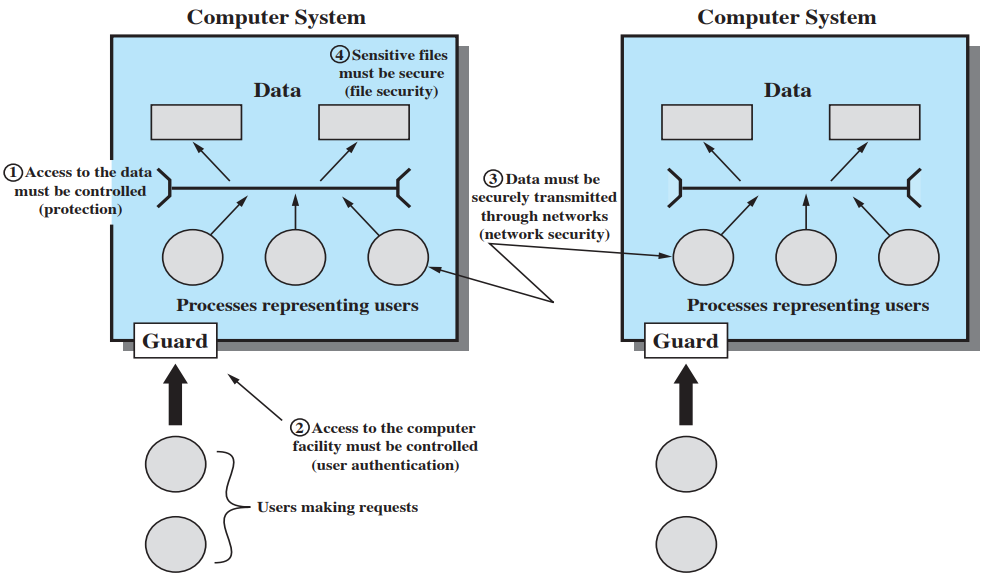
\includegraphics[scale=0.60]{img/scope.PNG}
					\caption{The	scope	of	computer	security\label{fig:4}}
				\end{figure}
		\subsection{Functional requirement per la sicurezza}
				Le contromisure possono essere classificate in termini di \textbf{requisiti funzionali}, prendiamo ad esempio lo standard FIPS200 che definisce 17 aree che coinvolgono misure tecniche per la sicurezza dei sistemi piuttosto che controlli e procedure di gestione.\\
				 \textit{Segue figure:\ref{fig:5}}
				\begin{figure}[h!]
					\centering
					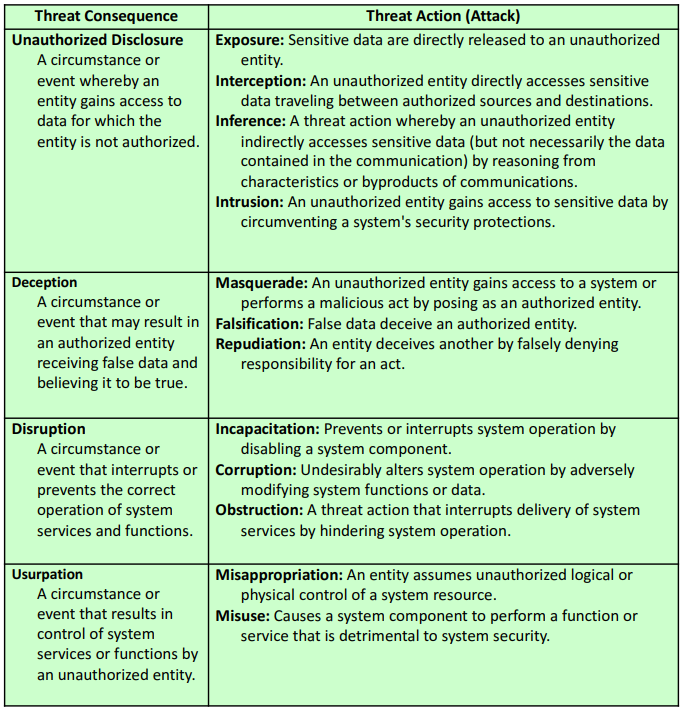
\includegraphics[scale=0.60]{img/threat.PNG}
					\caption{Threat consequences and attack\label{fig:5}}
				\end{figure}
				Ne elenchiamo alcune di rilievo:
				\begin{itemize}
					\item \textbf{Access Control (controllo accessi)}: limitare l'accesso alle informazioni del sistema ad utenti autorizzati, limitare i processi che agiscono per contro di utenti autorizzati, limitare il tipo di transazioni e funzioni che un utente autorizzato può utilizzare.
					\item \textbf{Awarness and Training (consapevolezza e addestramento) }: Assicurarsi che i manager e gli utenti del sistema siano informati riguardo ai rischi per la sicurezza associati alla propria attività, oltre alle leggi, regolamenti e politiche che riguardano la sicurezza di un sistema informativo. Inoltre ci dobbiamo assicurare che il personale sia ben addestrato per poter svolgere i propri doveri e responsabilità relativi alla sicurezza delle informazioni.
					\item \textbf{Incident response}: stabilire delle capacità operazionali che permettano la gestione di incidenti dovuti alla sicurezza dei dati. Include: preparazione, analisi, contenimento e ripristino. Risulta importante la capacità di tracciare, documentare e gli incidenti di sicurezza, con lo scopo di informare le autorità competenti.
				\end{itemize}
				Il concetto fondamentale riportato dal framework è quello di \textbf{combinare approcci tecnici e manageriali}.\\
				
				\textit{\textbf{“If you think technology can solve your security problems, then you 
					don’t understand the problems and you don’t technology”} }
		\subsection{Principi fondamentali di design per la sicurezza}
		
		\begin{figure}[h!]
			\centering
			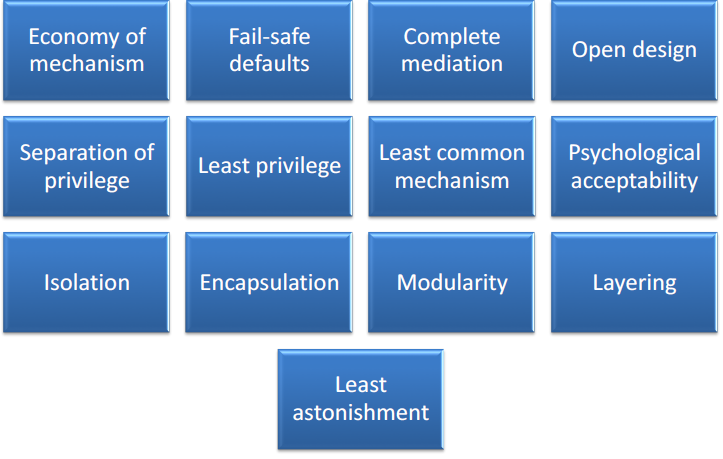
\includegraphics[scale=0.40]{img/desprinc.PNG}
			\caption{Fundamental security design principles\label{fig:6}}
		\end{figure}
			A dispetto di anni di ricerca, è ancora molto difficile progettare sistemi per i quali si possono sistematicamente escludere difetti e che siano in grado di prevenire azioni non autorizzate. Tuttavia sono state documentate delle \textbf{good practice} per una corretta progettazione di questi sistemi. Principi di design per la sicurezza che siano largamente accettati possono guidare l'implementazione dei meccanismi di sicurezza, inoltre possono fornire un \textbf{secondo punto di vista} riguardo le misure da adottare nei confronti di specifiche minacce al sistema.  \\
			\textit{Segue figure:\ref{fig:6}} \\
			\textit{Il National Centers of Academic Excellence in Information Assurance/Cyber Defense} elenca i relativi principi fondamentali: \\
			\begin{itemize}
				\item \textbf{Economy of mechanism (economia dei meccanismi):} il design delle misure di sicurezza devono essere più semplici possibile. Infatti più sono facili da implementare e testabili meno falle di sicurezza sono esposte.
				\item \textbf{Fail safe as default}: La gestione degli accessi deve essere basata sui permessi e la situazione di deafault deve essere quella di \textbf{negare l'acesso}. Infatti un meccanismo che fornisce permessi espliciti tende a fallire rifiutando gli accessi, una situazione sicura che può essere facilmente individuata.
				\item \textbf{Complete mediation}: Tutte le richieste di accesso devono passare per il meccanismo di controllo degli accessi. Nello specifico \textbf{non dobbiamo basare tali decisioni su eventuali cache degli accessi.}  
				\item \textbf{ Open Design:} Il design dei meccanismi di sicurezza deve essere open. Un esempio dei vantaggi ottenuti riguarda gli algoritmi per la criptografia: in questo modo possono essere analizzati e studiati da esperti, con lo scopo di migliorarne le prestazioni e la sicurezza.
				\item \textbf{Separation of privilege}: Dovrebbero essere necessari più privilegi per eseguire l'accesso o l'esecuzione di un'operazione. Esempio: \textbf{Autenticazione degli utenti a più fattori} (chiave odt + PIN). 
				\item \textbf{Least privilege}: Gli utenti devono avere privilegi minimi in relazione ai task che devono svolgere. In questo caso si evidenzia anche un aspetto temporale: un amministratore che ha privilegi speciali deve avere quei privilegi solo per il tempo necessario, quando eseguono attività ordinarie quei privilegi devono essere declassati.
				\item \textbf{Least common mechanism}: il design deve minimizzare le funzioni condivise da utenti diversi e quindi ridurre il numero di path di comunicazione indesiderati.
				\item \textbf{Psycological acceptability}: I meccanismi di sicurezza dovrebbero riflettere il modello mentale di protezione degli utenti. Il concetto è che i meccanismi di sicurezza non devono interferire impropriamente con il lavoro degli utenti.
				\item \textbf{Isolation:} legata a tre aspetti:
				\begin{enumerate}
					\item \textbf{Gli accessi pubblici dovrebbero essere isolati dalle risorse critiche in modo tale da prevenire disclosure o tampering (manomissioni).} \textit{A lezione è stato fatto l'esempio di \textbf{zona demilitarizzata}}.	
					\item I processi ed i file di uno specifico utente devono essere isolati l'uno rispetto all'altro.
					\item I meccanismi di sicurezza dovrebbero essere isolati.
				\end{enumerate}
				\item \textbf{Incapsulamento:} Una collezione di procedure e data ojects sono incapsulati in un dominio a se stante, così facendo la struttura interna di un oggetto solo dalle procedure del sottosistema protetto e le procedure possono essere chiamate solo agli entrypoint del dominio.
				\item \textbf{Modularity:} Abbiamo due significati :
				\begin{enumerate}
					\item Risulta opportuno che le funzioni di sicurezza siano sviluppate separatamente, come moduli protetti. Ad esempio, nel caso di un insieme di protocolli o applicazioni che utilizzano funzioni crittografiche, è opportuno che tali funzioni siano sviluppate in un comune modulo di crittografia che può essere invocato da tali funzioni, anzichè implementarle per ogni protocollo o applicazione.
					\item Il secondo riguarda la possibilità di sviluppare il design e l'implementazione dei meccanismi di sicurezza in senso modulare, in questo modo si possono aggiornare o modificare tali moduli senza dover modificare tutto il sistema.
				\end{enumerate}
				\item \textbf{Layering:} Utilizzare approcci sovrapposti alla sicurezza (più di uno) riguardo persone, tecnologia, e aspetti operazionali di un sistema informativo. In questo modo il fallimento di uno tra questi non lascerà il sistema privo di protezione (\textbf{defense in depth}: approccio militare per il quale si cerca di ritardare l'avanzata di un attaccante invece che prevenirla).
				\item \textbf{Leas astonishment:} Un programma o un'interfaccia deve rispondere in un modo per il quale è meno probabile che l'utente sia disorientato (stupito).
			\end{itemize}
		\subsection{Superfici di attacco e alberi di attacco}
			Ci fornisce un terzo punto di vista riguardo le misure che possono essere prese per gestire le minacce alla sicurezza di un sistema. 
			 \textit{Segue figure:\ref{fig:7}}
			\begin{figure}[h!]
				\centering
				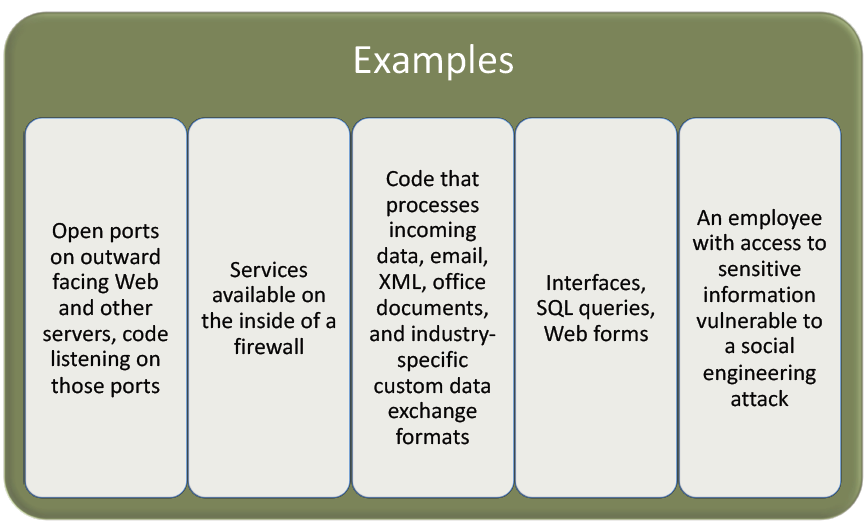
\includegraphics[scale=0.40]{img/exarea.PNG}
				\caption{Some reachable and exploitable vulnerabilities in a system\label{fig:7}}
			\end{figure}
			\subsubsection{Categorie di superfici di attacco}
				\begin{itemize}
					\item \textbf{Network attack surface}: Vulnerabilità che riguardano una rete aziendale, una rete su larga scala (wide-area network) oppure l'internet. Si includono vulnerabilità nei protocolli di rete utilizzate per attacchi denial-of-service e altri.
					\item \textbf{Software attack surface}: Vulnerabilità che riguardano in programmi e sistemi operativi ( con un riguardo particolare nei confronti del software dei web server).
					\item \textbf{Human attack surface}: Vulnerabilità create dal personale o da esterni (ingegneria sociale, errori umani e insider fidati). 
				\end{itemize}
				Un'\textbf{analisi della superficie di attacco} è utile nell'ottica di stabilire la scala e la severità delle minacce a cui un sistema è sottoposto. Una volta che la superficie di attacco è stata definita, \textbf{si può cercare di ridurla.}
			\subsubsection{Alberi di attacco}
				Un \textbf{albero di attacco} è una struttura dati ramificata (branching) e gerarchica che rappresenta un insieme di potenziali vulnerabilità. \textbf{L'obiettivo} è quello utilizzare in modo efficace (sfruttare/exploit) tutte le informazioni disponibili sui \textbf{pattern di attacco}. Infatti gli analisti della sicurezza possono utilizzare gli attack trees per guidare sia il design del sistema e delle applicazioni, oltre che la scelta e la forza delle contromisure. La conoscenza riguardo i pattern di attacco è stata raccolta nel tempo e rappresenta uno strumento importante alla sicurezza. Ad esempio il CERT (Computer Emergency Response Team) è uno degli organismi che ha svolto, nel tempo, questo genere di attività.
				
				\begin{itemize}
					\item \textbf{L'obiettivo (goal)} di un attacco (incidente di sicurezza) è rappresentato come radice dell'albero 
					\item \textbf{I modi (ways)} attraverso il quale l'attaccante può raggiungere un goal sono rappresentati iterativamente ed in modo incrementale come rami dell'albero.
					\item Ogni \textbf{sotto-nodo (subnode)} definisce un \textbf{sotto-obiettivo ( subgoal)}. Questo tipo di scomposizione di goal è ricorsiva.
					\item Le \textbf{foglie ( leaf nodes)} dell'albero rappresentano i diversi modi di \textbf{iniziare} un attacco
					\item Tutti i nodi escluse le foglie può essere un \textbf{And-node} oppure un \textbf{Or-node}.
					\begin{enumerate}
						\item Per realizzare un goal relativo ad un And-node si devono realizzare \textbf{tutti} i suoi subgoal.
						\item Per realizzare un goal relativo ad un Or-node si deve realizzare \textbf{almeno uno} dei suoi subgoal (Or non esclusivo).
					\end{enumerate} 
					\item I rami possono essere \textbf{etichettati }con valori rappresentati: difficoltà, costo o altri attributi in questo modo possiamo confrontare attacchi alternativi
				\end{itemize}
			\subsubsection{Albero di attacco relativo a una applicazione di autenticazione per servizio bancario }
				\begin{itemize}
					\item La radice rappresenta l'obiettivo dell'attaccante: \textbf{compromettere l'account di un utente}
					\item I \textbf{box verdi} sono gli eventi che costituiscono un attacco.
					\item I \textbf{box bianchi} sono categorie relative agli attacchi.
					\item Tutti i nod, tranne i nodi foglia, sono or nodes.
					\item L'analisi utilizzata per generare questo albero di attacco considera 3 componenti coinvolte nell'autenticazione.
					\begin{enumerate}
						\item \textbf{Terminali degli utenti e utenti (UT/U)}: questo genere di attacco mira agli strumenti utilizzati dagli utenti, inclusi i token coinvolti (smart card, password generator), oppure le azioni degli utenti.
						\item \textbf{Comunication channel (CC)}: Questi attacchi si concentrano sui canali di comunicazione.
						\item \textbf{Internet server bancari (IBS)}: questi sono attacchi offline nei confronti del server che ospita le applicazioni internet della banca. INSERIRE immagine pagina 63.
					\end{enumerate} 
				In questo scenario possiamo identificare 5 strategie di attacco che utilizzano una o più componenti delle tre identificate.
				\begin{itemize}
					\item \textbf{Credenziali utente compromesse}: consiste nel monitorare per osservare pin o credenziali dell'utente, rubare un token o una nota scritta a mano contenente un token, utilizzare programmi software malevoli per compromettere il login di un utente, hackerare una smart card, utilizzare un approccio a forza bruta per indovinare il pin di un utente, fare uno sniffing delle credenziali durante il loro passaggio in un canale di comunicazione.
					\item \textbf{Iniezione di comandi}: intercettare le comunicazioni tra un utente e il server della banca, impersonando quindi tale utente valido con lo scopo di ottenere l'accesso ai server della banca.
					\item \textbf{Indovinare le credenziali di un utente}: utilizzare algoritmi di forza bruta inviando login e password casuali.
					\item \textbf{Violazione delle politiche di sicurezza:} un dipendente può causare un incidente interno di sicurezza ed esporre l'account di un utente, se egli viola le politiche di sicurezza della banca in combinazione con un meccanismo di gestione degli accessi debole.
					\item \textbf{Utilizzare una sessione conosciuta già autenticata:} forzare un utente a connettersi al server della banca co un ID preimpostato, utilizzato dall'attaccante per rubare l'identità dell'utente.
				\end{itemize}
				\end{itemize}
			
		\subsection{Strategia per la computer security}
				Una strategia globale per provvedere alla sicurezza di un sistema:
			\begin{itemize}
				\item \textbf{Specifiche/politiche }: cosa dovrebbe fare lo schema di sicurezza ?
				\item \textbf{Implementazione/meccanismi:} come applicarli ?
				\item \textbf{Correttezza/assurance}: funziona davvero ?
			\end{itemize}
			\subsubsection{Specifiche/politiche}
				Dichiarazione formale di regole e pratiche che specificano e regolano come il sistema o un'organizzazione fornisce servizi di sicurezza, per proteggere le risorse critiche del sistema. I \textbf{fattori} da considerare nello sviluppare queste politiche sono:
				\begin{itemize}
					\item \textbf{Il valore delle risorse da proteggere};
					\item \textbf{Le vulnerabilità del sistema};
					\item \textbf{Potenziali minacce e la probabilità di subire un attacco}.
				\end{itemize}
				Si devono considerare anche i seguenti \textbf{trade-off}:
				\begin{itemize}
					\item \textbf{Facilità di utilizzo vs benefici di sicurezza};
					\item \textbf{Costo della sicurezza vs costi di fallimento e ripristino}
				\end{itemize}
				Inoltre queste politiche sono influenzate da \textbf{decisioni di business} e \textbf{requisiti legali}.
			\subsubsection{Implementazione/meccanismi}
				L'implementazione della sicurezza coinvolge quattro processi (courses of action) complementari:
				\begin{enumerate}
					\item \textbf{Prevenzione (Prevention)}: l'idea è che uno schema ideale di sicurezza è tale se nessun attacco ha successo. In qualche caso la prevenzione è un traguardo ragionevole. Es: attacchi alla confidentiality prevenuti utilizzando canali criptati.
					\item \textbf{Rilevazione (Detection)}: In alcuni casi, una protezione assoluta non è realizzabile, ma è molto più pratico rilevare gli attacchi alla sicurezza.
					\item \textbf{Reazione (Response)}: Il sistema può essere in grado di reagire in modo tale da bloccare un attacco alla sicurezza che è stato rilevato e prevenire così ulteriori danni.
					\item \textbf{Ripristino (Recovery)}: Se l'integrità dei file risulta compromessa è utile averne una copia corretta da poter ricaricare.
				\end{enumerate}
			\subsubsection{Correttezza/assurance}
\section{CryptoTools}
	Gli algoritmi crittografici sono una componente importante per la computer security. In questo capitolo si presenta una panoramica dei diversi tipi di algoritmo, ne discuteremo il contesto di applicazione e introdurremo gli algoritmi di uso comune più importanti.
	\subsection{Symmetric Encryption}
		La criptografia simmetrica risale agli anni 70 e per questo è anche indicata come \textbf{criptografia convenzionale} o criptografia a singola chiave. Nella pratica è una tecnica universale per fornire la \textbf{confidentiality} dei dati (trasmessi o salvati). Questo tipo di criptografia è ad oggi ancora la più utilizzata.
		\subsubsection{Model of Symmetric Encryption}
			Le componenti del modello sono le seguenti:
			\begin{enumerate}
				\item \textbf{Encryption algorithm}: esegue le sostituzioni e le trasformazioni sul plaintext.
				\item \textbf{Input}: 
					\begin{itemize}
						\item \textbf{Plaintext}: il messaggio originale da criptare.
						\item \textbf{Secret key}: le sostituzioni e le trasformazioni eseguite dall'algoritmo dipendono da questa chiave. Due chiavi segrete diverse produrranno due.
					\end{itemize} 
				\item \textbf{Ciphertext}: testo cifrato prodotto come \textbf{output} dall'algoritmo di encryption.
				\item \textbf{Decryption algorithm}: lavora al contrario dell'algoritmo di encryption (testo cifrato --- plain text).
			\end{enumerate}	
			INSERIRE IMMAGINE PAGINA 7
			I \textbf{requisiti} per un uso sicuro sono i seguenti:
			\begin{enumerate}
				\item è necessario un algoritmo di encryption che sia \textbf{forte}. Ciò significa che un attaccante \textbf{non deve essere in grado} di scoprire la chiave, nemmeno se è in possesso di un insieme di coppie cyphertext, plaintext.
				\item  Il sender e il receiver devono aver ottenuto la chiave in modo sicuro, si deve inoltre mantenerla sicura.
			\end{enumerate}
			I più diffusi algoritmi di symmetric encryption si basano su \textbf{block ciphers}. Block ciphers processa il plaintext in input in \textbf{blocchi di grandezza fissata} e produce in output blocchi di cyphertext della stessa grandezza. I principali algoritmi simmetrici (block ciphers) sono:
			\begin{itemize}
				\item DES
				\item Triple DES
				\item AES
			\end{itemize}
			INSERIRE IMMAGINE SLIDE 11
		\subsubsection{Approaches to Attacking}
			Gli approcci all'attacco riguardo la criptografia simmetrica sono due:
			\begin{enumerate}
				\item \textbf{Cryptanalitic Attacks}: si basa sulle caratteristiche dell'algoritmo. Si tenta di dedurre uno specifico plaintext o la chiave utilizzata (in questo ultimo caso non solo tutti i messaggi già inviati sono compromessi, ma anche quelli futuri). Si cerca di dedurre informazioni da coppie di plain e cyphertext.
				\item \textbf{Brute-Force Attacks}: Si prova a decifrare un cyphertex tentando tutte le chiavi possibili, fino a che non si ottiene un plain text che sia sensato. In media per aver successo si devono provare almeno la metà di tutte le chiavi possibili. Inoltre dobbiamo conoscere almeno una parte del plaintext per decidere se quello che otteniamo non è semplicemente unt testo senza senso (garble).
			\end{enumerate}
		\subsubsection{Data Encryption Standard (DES)}
			Adottato nel 1977 dal NIST, fino a poco tempo fa era l'algoritmo più utilizzato.
			\begin{enumerate}
				\item Prende in input\textbf{ blocchi di plaintext di 64 bit} e una \textbf{chiave da 56 bit} per produrre un \textbf{cyphertext da 64 bit.} 
				\item La chiave è anch'essa da 64 bit, ma 8 bit sono utilizzati per il \textbf{parity check}.
				\item L'algoritmo originariamente aveva chiavi da 128 bit che però sono state ridotte a 64 dal NIST.
			\end{enumerate}
		Analizziamo le \textbf{debolezze} dell'algoritmo dal punto di vista degli approcci di attacco visti in precedenza.
		\begin{itemize}
			\item Dal punto di vista delle debolezze dell'algoritmo (\textbf{cryptanalysis}), il DEA è uno dei più studiati tra gli algoritmi di encryption. Non sono mai state evidenziate debolezze critiche.
			\item La lunghezza delle chiavi è \textbf{56 bit} pertanto si ha un numero di $2^{56} $ chiavi possibili. La lunghezza delle chiavi rappresenta la debolezza maggiore, infatti l'algoritmo è stato violato nel 1998 dalla Electronic Frontier Foundation.
		\end{itemize}
		\textbf{\textit{Se l'unico modo di attaccare un algoritmo di enryption è quello di utilizzare brute force, allora la metodologia di difesa è ovvia: utilizzare chiavi più lunghe}}. 
		INSERIRE IMMAGINE PAGINA 14.
		\subsubsection{Triple DES}
			\begin{enumerate}
				\item Ripete tre volte l'algoritmo DES
				\item Si utilizzano 1,2 o 3 chiavi.
				\item La dimensione delle chiavi è di 168 bit.
			\end{enumerate}
			INSERIRE IMMAGINe PAG 15
			Vantaggi e svantaggi rispetto a \textbf{DES}:
			\begin{itemize}
				\item \textbf{Vantaggi:}
				\begin{enumerate}
					\item le chiavi a 168 bit permettono di superare le vulnerabilità rispetto a brute force ( anche se a sicurezza effettiva corrisponde a 112 bit).
					\item L'algoritmo sottostante è lo stesso di DES per il quale, come già detto non sono state individuate vulnerabilità critiche.
				\end{enumerate}
				\item \textbf{Svantaggi:} 
				\begin{enumerate}
					\item Il codice che implementa l'algoritmo non è efficiente ( computazionalmente oneroso).
					\item utilizza blocchi di \textbf{64 bit}, mentre sarebbero desiderabili blocchi di dimensioni maggiori, dal punto di vista della sicurezza e dell'efficienza.
				\end{enumerate}  
			\end{itemize}
		\subsubsection{Advanced Encryption Standards (AES)}
			Rimpiazza il 3DES. Requisiti definiti dal NIST:
			\begin{itemize}
				\item Sicurezza pari a 3DES.
				\item Efficienza significativamente migliorata.
				\item Symmetric block cipher.
				\item Blocchi di 128 bit.
				\item Chiavi da 128/192/256 bit.
			\end{itemize}
		\subsubsection{Block Cipher}
			Un plaintext ha una lunghezza di $n*b$ è diviso in n blocchi da b-bit. Nel caso la dimensione del plaintext non sia un multiplodi b si "imbottisce" il file aggiungendo bit. Ogni blocco è criptato separatamente. Produce una sequenza di n b-bit. \\
			\textbf{Electronic CodeBook} èl'approccio più semplice per l'encryption con blocchi multipli. Si utilizza l'algoritmo con una \textbf{stessa chiave per ogni blocco}. Questo approccio rende possibile applicare la cryptanalysis per individuare delle regolarità nel plaintext, pertanto potrebbe non essere indicato per messaggi di grossa lunghezza. \\
			INSERIRE IMMAGINE PAGINA 20\\
		\subsubsection{Stream Cipher Encryption}
			Uno stream cipher processa gli input in modo continuo producendo un output un elemento alla volta. Nello specifico \textbf{l'algoritmo cripta il plaintext un byte alla volta} (la lunghezza può essere configurata: ad esempio un bit alla volta). L'algoritmo effettua i seguenti passi:
			\begin{enumerate}
				\item Si utilizza uno pseudorandom bit generator, che prende in input la chiave di cifratura, che produce uno stream di numeri a 8 bit che sono apparentemente casuali.
				\item L'output di questo generatore, chiamato \textbf{keystream}, è combinato un byte alla volta con lo stream del plaintext utilizzando un l'operatore \textbf{XOR}.
			\end{enumerate}
			INSERIRE IMMAGINE PAGINA 22\\
		\subsubsection{Block Cipher vs Stream Cipher}
			\begin{itemize}
				\item Il vantaggio di block cipher è che si possono riutilizzare le chiavi.
				\item Il vantaggio di stream cipher è essere più veloce rispetto alla controparte, inoltre è necessario meno codice per l'implementazione.
				\item Se il generatore di numeri casuali è realizzato propriamente lo stream cipher può essere sicuro al pari di block cipher (a parità di lunghezza delle chiavi).
				\item block cipher è più appropriato per applicazioni che devono gestire blocchi di dati (trasferimento file, email, database). Al contrario è utilizzato nel caso di stream di dati (canali di comunicazione, browser).
			\end{itemize}
			In generale entrambi possono essere utilizzati in qualsiasi applicazione.
	\subsection{Message Authentication and Hash Function}
		\subsubsection{Message (or Data) Authentication}
			La message authentication fornisce protezione nei confronti di attacchi \textbf{attivi} (falsificazione dei dati), mentre la criptografia ci protegge da attacchi \textbf{passivi} (eavesdropping).\\
			La message authentication \textbf{è una procedura che permette alle parti coinvolte in una comunicazione di verificare che i messaggi ricevuti o salvati siano autentici} ovvero: 
			\begin{itemize}
				\item \textbf{genuini}: i contenuti non sono stati alterati.
				\item provengono dalla fonte attesa.
				\item \textbf{timeliness}: i messaggi non sono stati volontariamente ritardati o inviati una seconda volta (replay).
				\item \textbf{sequenza relativa} dei messaggi che vengono scambiati dalle due parti.
			\end{itemize}
			Tutti questi concerns riguardano \textbf{l'integrità dei dati}
		\subsubsection{Authentication with and without Symm. Encryption}
			\textbf{Nel caso di utilizzo della criptografia simmetrica}, se solo il sender e il receiver condividono la chiave allora:
			\begin{itemize}
				\item Solo il sender originale sarà in grado di fare l'encription di un messaggio ricevuto e depcriptato dal receiver.
				\item Se il messaggio include un codice per la \textbf{error detection} e un \textbf{sequence number}, il receiver è assicurato del fatto che nessuno modifica è stata apportata al file e che l'ordine relativo è giusto.
				\item Se il messaggio ha un timestamp il receiver è certo che il messaggio non sia stato ritardato di proposito.
			\end{itemize}
		\textbf{Tuttavia la criptografia simmetrica non è un tool adatto per la data authentication}. Infatti se un attaccante riordina i blocchi di un singolo ciphertext, i blocchi vengono comunque decriptati con successo. Tuttavia l'ordinamento posticcio dell'attaccante fa si che il testo decriptato perda il suo significato.   \\
		Nel caso in cui non si utilizzi criptografia simmetrica l'approccio è quello di utilizzare un \textbf{authentication tag} che viene allegato in ogni messaggio. In questo caso \textbf{non si garantisce la confidentiality} dei dati ma solo \textbf{l'autenticazione}. Ovviamente è possibile combinare i due approcci in un solo algoritmo.\\
		Tuttavia le funzioni che realizzano la message authentication e l'encryption sono tenute separate poichè ci sono situazioni in cui, tra le due, l'encryption è superflua:
		\begin{itemize}
			\item Applicazioni nelle quali un messaggio deve essere inviato tramite \textbf{broadcast} a più destinatari. In questo caso è molto meno oneroso avere un solo destinatario responsabile di monitorare l'autenticità. Si invia tramite broadcast un plaintext con un authentication tag, dunque il sistema responsabile di eseguire l'autenticazione verifica che ci siano violazioni ed in caso positivo avvisa tutti gli altri destinatari.
			\item Scenario nel quale due entità si scambiano dati e uno dei due ha un \textbf{grosso carico di lavoro} a causa del quale non ha tempo per 	decriptare tutti i messaggi in entrata.
			\item Un altro scenario è quello dell'\textbf{esecuzione di un programma}. Il programma può essere eseguito senza che il suo codice debba essere decriptato ogni volta (oneroso per il processore). Avere un authentication tag ci permette di controllare comunque \textbf{l'integrità} del programma (se richiesto). 
		\end{itemize}
		\subsubsection{Message Authentication Code (MAC)}
			Un'altra tecnica di autenticazione è quella di utilizzare un blocco di dati di piccole dimensioni (MAC) da allegare al messaggio e generato utilizzando una chiave segreta condivisa tra mittente e destinatario. Nello specifico:
			\begin{enumerate}
				\item Quando A ha un messaggio per B, calcola il MAC come una funzione complessa del messaggio e della chiave $MAC_{M} = F(K_{AB},M)$.
				\item Si trasmette il messaggio più il MAC a B.
				\item B esegue lo stesso calcolo utilizzando il messaggio e la chiave e producendo quindi un altro MAC.
				\item Il MAC spedito da A viene confrontato da B con quello da lui generato. 
			\end{enumerate}
			Le proprietà che garantisce questo sistema di sicurezza, se la chiave è conosciuta solo da A e B e i MAC corrispondono, sono le seguenti:
			\begin{itemize}
				\item Il destinatario ha la garanzia che il messaggio \textbf{non sia stato alterato}
				\item Il destinatario ha la garanzia che il messaggio \textbf{proviene dal mittente atteso}.
				\item Se il messaggio contiene un timestamp si può garantire \textbf{ordine relativo e timeliness}.
			\end{itemize}
		
			INSERIRE IMMAGINE PAGINA 31\\
			Alcune \textbf{considerazioni}: un codice MAC da 16 - 32 bit attualmente non garantisce la \textbf{collision resistance}. Una funzione H è collision resistance se è difficile trovare due input che sono mappati sullo stesso output. Ovviamente una funzione che ha più input che output (dominio$>$ codominio) avrà delle collisioni, la collision resistance significa che le collisioni sono \textbf{difficili da trovare}.\\
			Un'altra considerazione è che, a differenza dell'encryption, l'algoritmo di autenticazione non deve essere \textbf{reversibile}.
		\subsubsection{Cryptographic Hash Function}
			Si possono utilizzare \textbf{one-way hash function} per l'authentication. Una funzione hash accetta un messaggio M di lunghezza variabile e produce in output un \textbf{digest H(M)} di lunghezza fissata. Al messaggio è abbinato un multiplo di una lunghezza fissata a cui a sua volta è associato un parametro L che indica la lunghezza del messaggio originale. Il parametro L è una difficoltà in più per un attaccante nell'ottica di produrre un messaggio alternativo con lo stesso valore hash. \textbf{A differenza del MAC non utilizza una chiave segreta come input}.\\
			\textbf{Non solo il digest garantisce l'authentication, ma anche la data integrity} ( indfatti se un qualche bit risulta alterato il digest darà un errore).\\
			INSERIRE IMMAGINE PAGINA 34\\
			INSERIRE IMMAGINE PAGINA 36\\
			INSERIRE IMMAGINE PAGINA 37\\
			INSERIRE IMMAGINE PAGINA 38\\
			FINIRE HASH FUNCTION
	\subsection{Public Key Encryption}
		Proposta da Diffie e Hellman nel 1976 rappresenta un avanzamento rivoluzionario della tecnologia criptografica.\\
		Gli \textbf{ingredienti} di questo tipo di criptografia sono:
		\begin{itemize}
			\item Come al solito un \textbf{plaintext} ed il relativo \textbf{ciphertext}, ottenuto dal primo tramite un \textbf{algoritmo di encryption}. Ovviamente sarà necessario anche un algoritmo di \textbf{decriptazione}.
			\item Una coppia di chiavi una \textbf{pubblica} e una \textbf{privata}, una sarà utilizzarta per criptare il plaintext l'altra per decriptarlo (dipende dallo scopo e da quale si sceglie.)
		\end{itemize}
		Ci sono diverse \textbf{false idee} riguardo la criptografia con chiave pubblica rispetto a quella simmetrica:
		\begin{itemize}
			\item \textbf{più sicura:} non c'è alcuna differenza in relazione alla restistenza alla cryptanalysis, tra criptografia simmetrica e a chiave pubblica
			\item \textbf{rende criptografia simmetrica obsolete}: La criptografia a chiave pubblica ha un overhead computazionale considerevole rispetto alla controparte simmetrica, pertanto non c'è motivo per il quale la prima dovrebbe sostituire l'altra.
		\end{itemize}
		Possiamo criptare un messaggio utilizzando la chiave pubblica o quella privata, analizziamo questi due scenari.\\
		\subsubsection{Encryption with public key}
			Per l'\textbf{encryption con chiave pubblica} il procedimento è il seguente:
			\begin{enumerate}
				\item Ogni utente genera una coppia di chiavi, una pubblica l'altra privata. La chiave pubblica è salvata in un registro accessibile agli altri, mentre la chiave privata è tenuta segreta.
				\item Se Bob vuole inviare un messaggio ad Alice, \textbf{utilizza la chiave pubblica di Alice per criptare il messaggio.}
				\item Quando Alice riceve un messaggio lo \textbf{decripta utilizzando la sua chiave privata}. Nessun altro potrà decriptare il messaggio poichè la chiave pubblica di alice, utilizzata per l'encryption, si abbina solo a quella privata di quest'ultima (che solo lei conosce).
				\item La distribuzione delle chiavi è più semplice rispetto all'handshaking della controparte simmetrica: le procedure non sono più semplici. 
			\end{enumerate}
		\subsubsection{Encrytpion with private key}
			Per questo motivo tale schema di encryption \textbf{è utilizzato con lo scopo di garantire la confidentiality} di un messaggio. Ovviamente la confidentiality che è garantita dipende da diversi fattori, tra i quali la sicurezza dell'algoritmo, se la chiave privata è tenuta al sicuro e la sicurezza del protocollo di cui la funzione di encryption fa parte.\\
			INSERIRE IMMAGINE PAGINA 47\\
			Alternativamente possiamo effettuare l'\textbf{encryption del messaggio con la chiave privata}, attraverso il seguente procedimento:
			\begin{enumerate}
				\item Bob cripta il messaggio con la propria chiave privata 	
				\item chiunque conosca la sua chiave pubblica può decriptare il messaggio.
			\end{enumerate}
			Questo schema di encryption è utilizzato per \textbf{garantire l'authentication e/o la data integrity}:
			\begin{itemize}
				\item Se qualcuno è in grado di decriptare un messaggio utilizzando la chiave pubblica di Bob è sicuro che quel messaggio provenga da bob, poichè solo la chiave privata di Bob avrebbe potuto criptare quel messaggio.
				\item Solo Bob può modificare il testo poichè le modifiche si possono fare esclusivamente con la chiave privata di bob.
				\item L'integrità e l'authentication dipendono dagli stessi fattori elencati per lo schema precedente.
			\end{itemize}
		\subsubsection{Requirement for Public-Key Cryptosystems and Algorithms}
			I requirements che vogliamo per questo tipo di criptografia sono i seguenti:
			\begin{itemize}
				\item facile a livello computazionale creare paia di chiavi
				\item facile reperire le chiavi pubbliche per criptare i messaggi
				\item facile per il receiver conoscere la chiave privata del sender
				\item impossibile per l'attaccante risalire alla chiave privata essendo a conoscenza della chiave pubblica.
				\item Infattibile a livello computazionale risalire al plaintext senza essere a conoscenza dalla chiave privata.
				\item Utile anche se non necessario per tutte le applicazioni poter utilizzare entrambe le chiavi sia per la decriptazione sia per la criptazione.
			\end{itemize}
			Di seguito un elenco di algoritmi di encryption a chiave pubblica (dettagli pagina 51 slide):
			\begin{itemize}
				\item \textbf{RSA}
				\item \textbf{Diffie-Hellman key exchange algorithm}
				\item \textbf{Digital Signature Standards (DSS)}
				\item \textbf{Elliptic curve cryptography}
			\end{itemize}
		Gli utilizzi per questi algoritmi sono i seguenti : INSERIRE IMMAGINE PAGINA 56.\\
	\subsection{Digital Signatures and Key Management}
		Gli algoritmi a chiave pubblica sono utilizzati per due categorie di applicazioni, le \textbf{Digital Signatures} e \textbf{Key management and distribution}. Gli aspetti che dobbiamo considerare riguardo queste due categorie sono:
		\begin{itemize}
			\item La distribuzione sicura delle chiavi pubbliche (\textbf{Public-Key Certificates})
			\item La distribuzione delle chiavi simmetriche 
			\item La protezione delle chiavi simmetriche one-time per l'encryption (Digital Envelopes).
		\end{itemize}
		\subsubsection{Digital Signature}
			Definita come \textbf{il risultato di una trasformazione criptografica di dati, che se propriamente implementata, mette a disposizione un meccanismo per verificare la sua autenticazione, l'integrità dei dati e il non ripudio da parte del firmatario.} \textbf{Pertanto consiste nel criptare un messaggio ottenuto dal plaintext con una chiave privata utilizzata come firma}.Supponiamo che Bob voglia inviare un messaggio ad Alice in modo che sia certo che il messaggio proviene da lui. Il funzionamento è il seguente:
			\begin{enumerate}
				\item Bob utilizza una hash function sicura per generare un \textbf{hash value per il messaggio}.
				\item L'\textbf{hash value insieme alla chiave privata} di Bob sono gli input per l'algoritmo che genera la firma digitale. L'output è un \textbf{blocchetto} che è utilizzato come firma digitale.
			\end{enumerate}
			Quando Alice riceve il messaggio :
			\begin{enumerate}
				\item Calcola un hash value per il messaggio
				\item utilizza questo hash value e la chiave pubblica di Bob per verificare che il messaggio provenga effettivamente da lui.
			\end{enumerate}
			In questo modo Alice è sicura che il messaggio arriva da Bob perchè:
			\begin{itemize}
				\item Un messaggio che è verificato tramite la chiave pubblica di Bob e l'hash del messaggio, ha una firma digitale creata necessariamente con la chiave private di Bob.
				\item Nessuno può modificare il messaggio senza conoscere la chiave privata di Bob, pertanto si garantisce anche la \textbf{data integrity}.
				\item Non si garantisce tuttavia la \textbf{confidentiality}. Infatti anche se il messaggio fosse completamente criptato (non solo l'hash) chiunque potrebbe decriptarlo utilizzando la chiave pubblica.
			\end{itemize}
			INERIRE IMMAGINE PAGINA 58\\
		\subsubsection{Public Key Certificates}
			Una delle principali \textbf{debolezze} della \textbf{public key encryption} riguarda il fatto che le \textbf{chiavi pubbliche possono essere falsificate}. Un qualche utente potrebbe infatti fingere di essere Bob e mandare mandare una chiave pubblica ad un altro partecipante o effettuare addirittura un broadcast di questa chiave. Prima che Bob si accorga della falsificazione e che informi gli altri partecipanti, il falsificatore è in grado di di leggere tutti i messaggi che gli altri utenti pensano di inviare a Bob ( infatti la chiave pubblica di un utente è utilizzata criptare messaggi a lui destinati).\\
			Una possibile soluzione è rappresentata dai \textbf{certificati a chiave pubblica}: Un certificato consiste in una \textbf{chiave pubblica e un user ID del proprietario della chiave}, inoltre il blocco formato dai due deve essere \textbf{firmato da una terza parte fidata}:
			\begin{itemize}
				\item Il certificato contiene informazioni riguardo la terza parte piu un'indicazione \textbf{del suo periodo di validità}.
				\item Comunemente la terza parte è \textbf{un'autorità certificata} come un'agenzia governativa o un'istituzione finanziaria.
				\item In pratica un utente può presentare in modo sicuro la sua chiave pubblica ed ottenere il relativo certificato dalla terza parte.
				\item A questo punto l'utente può pubblicare il proprio certificato.
				\item Chiunque voglia utilizzare la chiave pubblica può ottenere il certificato e verificarne la validità attraverso il garante di terze parti.
			\end{itemize} 
			L'\textbf{X.509 standard }è uno schema universalmente accettato per formattare i certificati a chiave pubblica, utilizzata nella maggior parte delle applicazioni di rete (ip security,transport layer security (TLS),Secure shell (SSH) ecc).
			INSERIRE IMMAGINE A PAGINA 62
		\subsubsection{Symmetric Key Exchange Using Public-Key Encryption}
			FUFFA (Guardare 64 per dettagli)
		\subsubsection{Digital Envelopes}
			Questa tecnica è utilizzata per proteggere la \textbf{confidenzialità} dei messaggi, \textbf{senza che i partecipanti alla comunicazione si debbano mettere d'accordo in precedenza sull'adozione di una chiave segreta condivisa.} Rappresenta l'equivalente di una raccomandata. Questa tecnica si sviluppa nei seguenti passaggi (supponendo che Bob voglia inviare un messaggio ad Alice):
			\begin{enumerate}
				\item Preparare il messaggio da inviare
				\item Generare una chiave simmetrica casuale che sarà utilizzata solo una volta.
				\item Utilizzare quella chiave per criptare il messaggio
				\item Utilizzare la chiave pubblica di Alice per criptare la chiave simmetrica 
				\item Allegare la chiave simmetrica criptata al messaggio criptato.
				\item Alice esegue i passaggi inversi, cominciando col dividere la chiave criptata dal messaggio criptato
				\item Decripta la chiave simmetrica utilizzando la propria chiave privata
				\item Decripta il messaggio utilizzando la chiave simmetrica ottenuta.
			\end{enumerate} 
			In questo modo solo Alice è in grado di decriptare la chiave simmetrica e dunque decriptare anche il messaggio (confidentiality). Se Bob ha ottenuto la chiave pubblica di Alice attraverso il certificato a chiave pubblica, sa che la chiave pubblica è valida e che dunque invierà il messaggio effettivamente ad Alice (authentication).\\
			INSERIRE IMMAGINE PAGINA 70\\
	\subsection{Random and Pseudorandom Numbers}
		I numeri casuali giocano un ruolo fondamentale nell'utilizzo dell'encryption.
			
			
		
		
			 
			 
			 	
	
		


\end{document}